\section{DROP: Workload Optimization}
\label{sec:algo}

In this section, we introduce DROP, a system that performs workload-aware DR via progressive sampling and online progress estimation.
DROP takes as input a target dataset, metric to preserve (default, target $TLB$), and an optional downstream runtime model.
DROP then uses sample-based PCA to identify and return a low-dimensional representation of the input that preserves the specified property while minimizing estimated workload runtime (Figure 2, Alg.~\ref{alg:DROP}).

%DROP answers a crucial question that stochastic PCA techniques have traditionally ignored: how long should these methods run? 

\begin{comment}
Notation used is in Table~\ref{table:inputs}.

\begin{table}
\centering
\small
\caption{\label{table:inputs} 
 DROP algorithm notation and defaults}
{\renewcommand{\arraystretch}{1.2}
\begin{tabular}{|c|l l|}
\hline 
Symbol & Description (\emph{Default}) & Type\tabularnewline
\hline
$X$  & Input dataset                          & $\mathbb{R}^{\mvar \times \dvar}$ \tabularnewline
$\mvar$  & Number of input data points            & $\mathbb{Z}_{+}$\tabularnewline
$\dvar$  & Input data dimension                   & $\mathbb{Z}_{+}$ \tabularnewline
$B$  & Target $TLB$ preservation      		 & $0 < \mathbb{R} \leq 1 $ \tabularnewline
$\mathcal{C}_\mvar(\dvar)$  & Downstream runtime function (\textit{k-NN runtime})       & $\mathbb{Z}_{+} \to \mathbb{R}_{+}$\tabularnewline
$R$  & Total DROP runtime       & $\mathbb{R}_{+}$ \tabularnewline
$c$ & Confidence level for $TLB$ preservation (\textit{$95 \%$})          & $\mathbb{R}$  \tabularnewline
$T_k$  & DROP output $k$-dimensional transformation &$\mathbb{R}^{\dvar \times k}$ \tabularnewline
$i $ & Current DROP iteration        & $\mathbb{Z}_+$  \tabularnewline

\hline 
\end{tabular}
}
\end{table}
\end{comment}

\begin{figure}
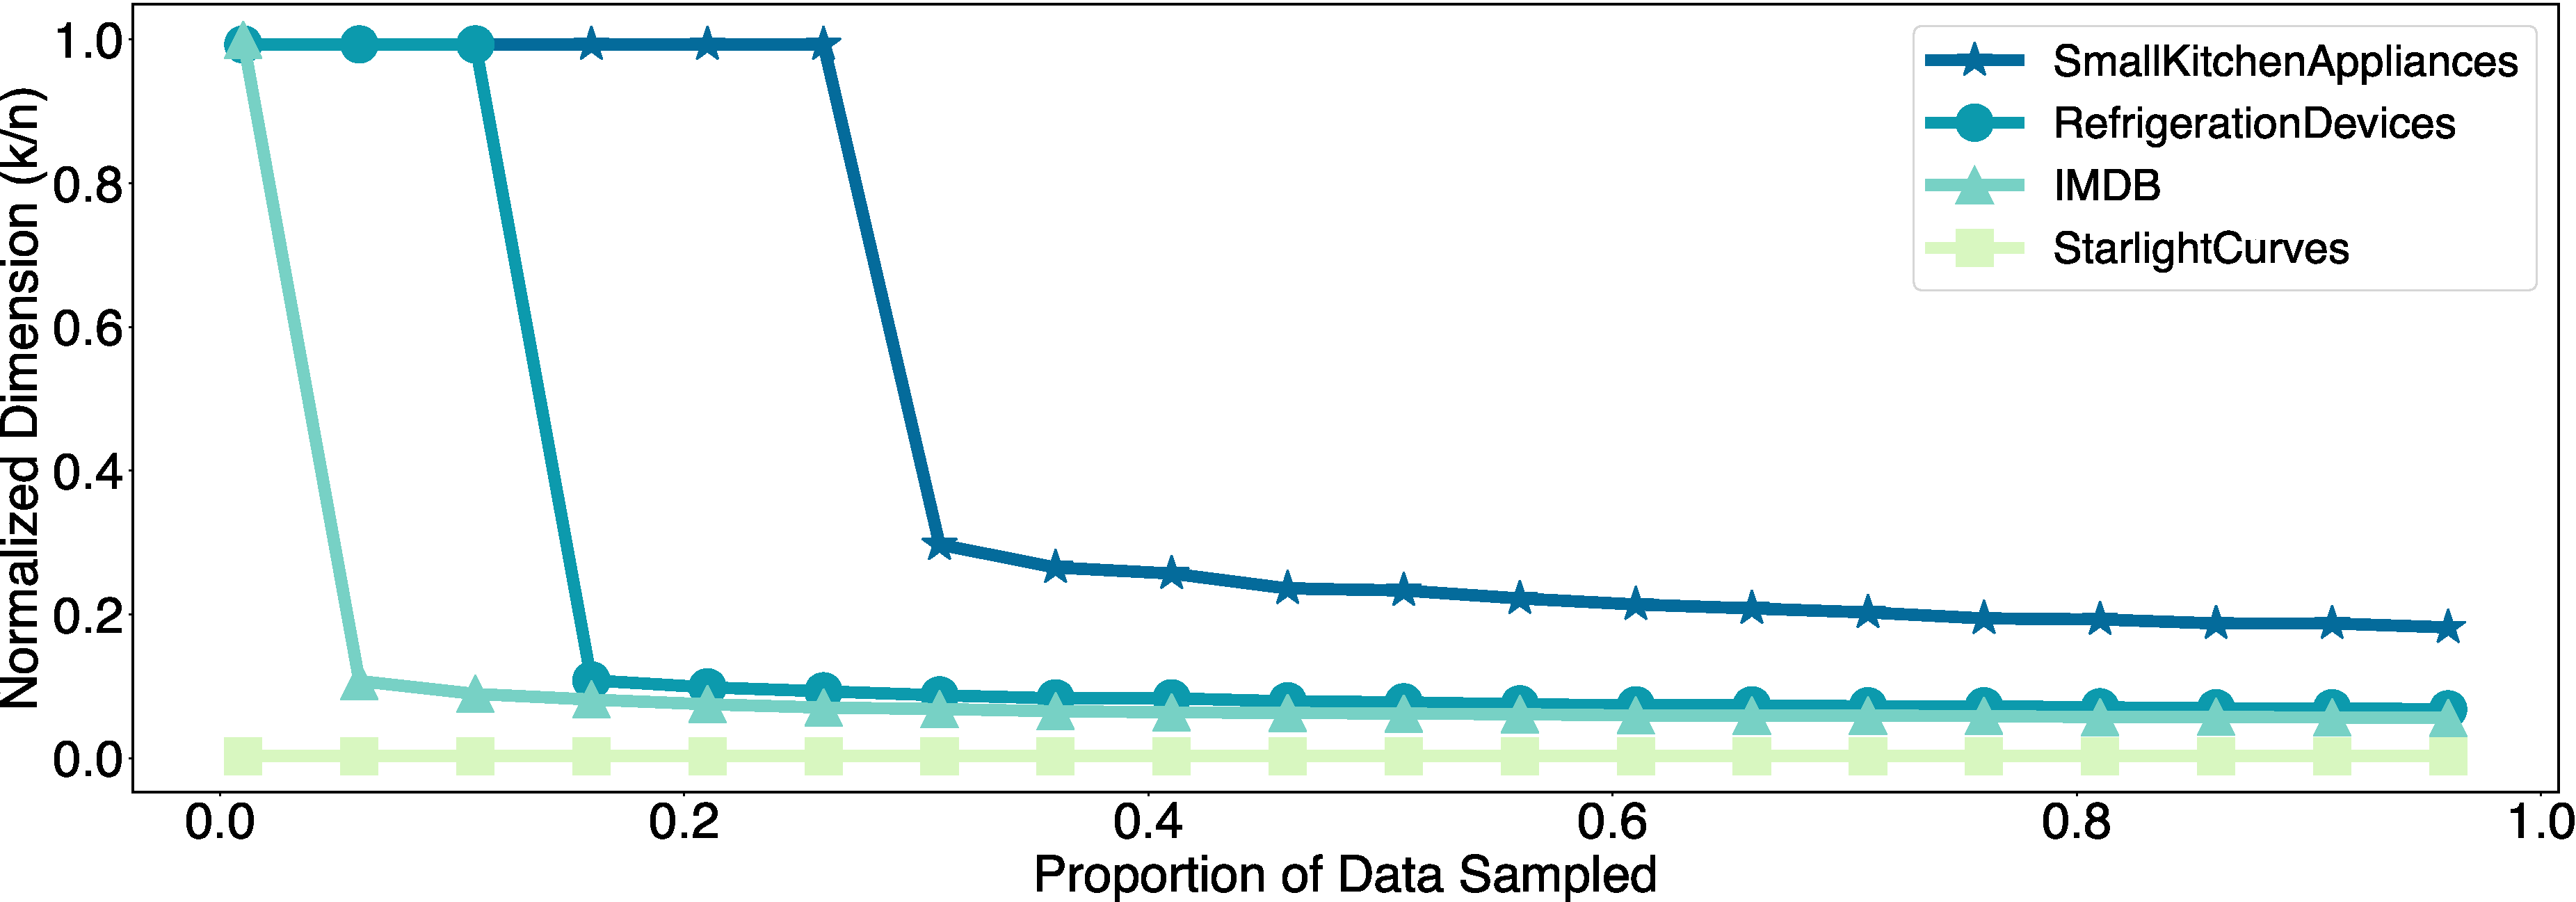
\includegraphics[width=\linewidth]{figs/progressive.pdf}
\caption[]{ Reduction in dimensionality for  $TLB = 0.80$ with progressive sampling. Dimensionality decreases until reaching a state equivalent to running PCA over the full dataset ("convergence").}
\label{fig:progressive}
\end{figure}

\subsection{DROP Algorithm}
\label{subsec:arch}
%DROP is a system that performs workload-aware dimensionality reduction, optimizing the combined runtime of downstream tasks and DR as defined in Problem~\ref{def:opt}.
DROP operates over a series of data samples, and determines when to terminate via \red{a} four-step procedure at each iteration: %progressive sampling, transformation evaluation, progress estimation, and cost-based optimization:

%To power this pipeline, DROP combines database and machine learning techniques spanning online aggregation (\S\ref{subsec:teval}), progress estimation (\S\ref{subsec:pest}), progressive sampling (\S\ref{subsec:psample}), and PCA approximation (\S\S\ref{subsec:pcaroutine},\ref{subsec:reuse}).

%We now provide a brief overview of DROP's sample-based iterative architecture before detailing each.

\begin{comment}
\item Progressive Sampling (\S\ref{subsec:psample}): DROP draws a data sample, performs PCA over it, and uses of a novel reuse mechanism across iterations (\S\ref{subsec:reuse}).

\item Transform Evaluation (\S\ref{subsec:teval}): DROP evaluates the above by identifying the size of the smallest metric-preserving transformation that can be extracted. 

\item Progress Estimation (\S\ref{subsec:pest}): Given the size of the smallest metric-preserving transform and the time required to obtain this transform, DROP estimates the size and computation time of continued iteration.

\item Cost-Based Optimization (\S\ref{subsec:opt}): DROP optimizes over DR and downstream task runtime to determine if it should terminate.
\end{comment}

\minihead{Step 1: Progressive Sampling (\S\ref{subsec:psample})}

\noindent DROP draws a data sample, performs PCA over it, and uses of a novel reuse mechanism across iterations (\S\ref{subsec:reuse}).

\minihead{Step 2: Transform Evaluation (\S\ref{subsec:teval})} 

\noindent DROP evaluates the above by identifying the size of the smallest metric-preserving transformation that can be extracted. 

\minihead{Step 3: Progress Estimation (\S\ref{subsec:pest})} 

\noindent Given the size of the smallest metric-preserving transform and the time required to obtain this transform, DROP estimates the size and computation time of continued iteration.

\minihead{Step 4: Cost-Based Optimization (\S\ref{subsec:opt})} 

\noindent DROP optimizes over DR and downstream task runtime to determine if it should terminate.

\subsection{Progressive Sampling}
\label{subsec:psample}

Inspired by stochastic PCA methods (\S\ref{sec:relatedwork}), DROP uses sampling to tackle workload-aware DR. 
Many real-world \red{datasets} are intrinsically low-dimensional; a small data sample is sufficient to characterize dataset behavior. 
To verify, we extend our case study (\S\ref{sec:RQW}) by computing how many uniformly selected data samples are required to obtain a $TLB$-preserving transform with $k$ equal to input dimension $\dvar$.
On average, a sample of under $0.64\%$ $(\text{up to } 5.5\%)$ of the input is sufficient for $TLB = 0.75$, and under $4.2\%$ $(\text{up to } 38.6\%)$ is sufficient for $TLB=0.99$.  
If this sample rate is known, we obtain up to \red{$91\times$ speedup} over PCA via SVD.%---with no algorithmic improvement. 

However, this benefit is dataset-dependent, and unknown a priori.
We thus turn to progressive sampling (gradually increasing the sample size) to identify how large a sample suffices.
Figure~\ref{fig:progressive} shows how the dimensionality required to attain a given $TLB$ changes when we vary dataset and proportion of data sampled.
Increasing the number of samples (which increases PCA runtime) provides lower $k$ for the same $TLB$.
However, this decrease in dimension plateaus as the number of samples increases.
Thus, while progressive sampling allows DROP to tune the amount of time spent on DR, DROP must determine when the downstream value of decreased dimension is overpowered by the cost of DR---that is, whether to sample to convergence or terminate early (e.g., at $0.3$ proportion of data sampled for SmallKitchenAppliances). 


Concretely, DROP first repeatedly chooses a subset of data and computes a $\dvar$-dimensional transformation via PCA on the subsample, and then proceeds to determine if continued sampling is beneficial to end-to-end runtime.
We consider a simple uniform sampling strategy: each iteration, DROP samples a fixed percentage of the data.
 
 
 
 
 
%Exploring data-dependent and weighted sampling schemes that are dependent on the current basis is an exciting area for future work. 
%While we considered a range of alternative sampling strategies, uniform sampling strikes a balance between computational and statistical efficiency. 
%Data-dependent and weighted sampling schemes that are dependent on the current basis may decrease the total number of iterations required by DROP, but may require expensive reshuffling of data at each iteration~\cite{coresets}. 

%DROP provides configurable strategies for both base number of samples and the per-iteration increment, in our experimental evaluation in \S\ref{sec:experiments}, we consider a sampling rate of $1\%$ per iteration.
%We discuss more sophisticated additions to this base sampling schedule in the extended manuscript.

\begin{algorithm}[t!]
\begin{algorithmic}[1]
\small
\Statex \textbf{Input:}  $X$: data; $B$: target metric preservation level; $\mathcal{C}_\mvar$: cost of downstream operations
\Statex \textbf{Output:} $T_k$: $k$-dimensional transformation matrix
\Statex
\Statex \hrule
\Function{drop}{$X,  B, \mathcal{C}_\mvar$}:
	\State Initialize: $i = 0; k_0 = \infty$ 
		\Comment{iteration and current basis size}
	\Do
		\State i$\texttt{++}$, \textsc{clock.restart}
		\State $X_i$ = \textsc{sample}($X, \textsc{sample-schedule}(i)$) \label{eq:sample}
			\Comment{\S~\ref{subsec:psample}}
		\State $T_{k_i}$ = \textsc{compute-transform}($X, X_i,  B$) \label{eq:evaluate}
			\Comment{\S~\ref{subsec:teval}}
		\State $r_i = \textsc{clock.elapsed}$	
			\Comment{$R = \sum_i r_i$}
		\State $\hat{k}_{i+1}, \hat{r}_{i+1} $ = \textsc{estimate}($k_i, r_i$) \label{eq:estimate}
			\Comment{\S~\ref{subsec:pest}}
	\doWhile{\textsc{optimize}($\mathcal{C}_\mvar,k_i,r_i,\hat{k}_{i+1}, \hat{r}_{i+1}$)} \label{eq:optimize}
		\Comment{\S~\ref{subsec:opt}}
	\\\Return{$T_{k_i}$}
\EndFunction
\end{algorithmic}
\caption{DROP Algorithm}
\label{alg:DROP}
\end{algorithm}



\subsection{Transform Evaluation}
\label{subsec:teval}
DROP must accurately and efficiently evaluate this iteration's performance with respect to the metric of interest \red{over the entire dataset}. 
%To do so, DROP adapts an approach for deterministic queries in online aggregation: treating quality metrics as aggregation functions and using confidence intervals for fast estimation. 
%We first discuss this approach in the context of $TLB$, then discuss how to extend this approach to alternative metrics at the end of this section.
We define this iteration's performance as the size of the lowest dimensional $TLB$-preserving transform ($k_i$) that it can return. 
There are two challenges in performance evaluation.
First, the lowest $TLB$-achieving $k_i$ is unknown a priori. 
Second, brute-force $TLB$ computation would dominate the runtime of computing PCA over a sample. 
We now describe how to solve these challenges.

\subsubsection{Computing the Lowest Dimensional Transformation}

Given the $\dvar$-dimensional transformation from step 1, to reduce dimensionality, DROP must determine if a smaller dimensional $TLB$-preserving transformation can be obtained and return the smallest such transform. 
Ideally, the smallest $k_i$ would be known a priori, but in practice, this is not true---thus, DROP uses the $TLB$ constraint and two properties of PCA to automatically identify it.
%A na\"ive strategy would evaluate the $TLB$ for every combination of the $\dvar$ basis vectors for every transformation size, requiring $O(2^\dvar)$ evaluations. 
%Instead, DROP exploits two key properties of PCA to avoid this.

First, PCA via SVD produces an orthogonal linear transformation where the principal components  are returned in order of decreasing dataset variance explained.
As a result, once DROP has computed the transformation matrix for dimension $\dvar$, DROP obtains the transformations for all dimensions $k$ less than $\dvar$ by truncating the matrix to $\dvar \times k$ .
%PCA via SVD produces an orthogonal linear transformation where the first principal component explains the most variance in the dataset, the second explains the second most---subject to being orthogonal to the first---and so on.  

Second, with respect to $TLB$ preservation, the more principal components that are retained, the better the lower-dimensional representation in terms of $TLB$.  
This is because orthogonal transformations such as PCA preserve inner products. 
Therefore, an $\dvar$-dimensional PCA perfectly preserves $\ell_2$-distance between data points. 
As $\ell_2$-distance is a sum of squared (positive) terms, the more principal components retained, the better the representation preserves $\ell_2$-distance.

Using the first property, DROP obtains all low-dimensional transformations for the sample from the $\dvar$-dimensional basis.  
Using the second property, DROP runs binary search over these transformations to return the lowest-dimensional basis that attains $B$ (Alg.~\ref{alg:candidate}, l\ref{eq:basis}).
If $B$ cannot be realized with this sample, DROP omits further optimization steps and continues the next iteration by drawing a larger sample.

Additionally, computing the full $\dvar$-dimensional basis at every iteration may be wasteful. 
Thus, if DROP has found a candidate $TLB$-preserving basis of size $\dvar' < \dvar$ in prior iterations, then DROP only computes $\dvar'$ components at the start of the next iteration.
This allows for more efficient PCA computation for future iterations, as advanced PCA routines can exploit the $\dvar'$-th eigengap to converge faster (\S\ref{sec:relatedwork}).
% \red{This is because similar to a hold-out or validation set, $TLB$ evaluation is representative of the entire dataset, not just the current sample (see Alg.~\ref{alg:candidate} L5). 
%Thus, sampling additional training datapoints enables DROP to better learn global data structure and perform at least as well as over a smaller sample.}


% stop here!

\subsubsection{Efficient $TLB$ Computation}

Given a transformation, DROP must determine if it preserves the desired $TLB$.
Computing pairwise $TLB$ for all data points requires $O(\mvar^2\dvar)$ time, which dominates the runtime of computing PCA on a sample.
However, as the $TLB$ is an average of random variables bounded from 0 to 1, DROP can use sampling and confidence intervals to compute the $TLB$ to arbitrary confidences.

Given a transformation, DROP iteratively refines an estimate of its $TLB$ (Alg.~\ref{alg:candidate}, l\ref{eq:eval}) by \red{incrementally sampling an increasing number of} pairs from the input data (Alg.~\ref{alg:candidate}, l\ref{eq:paircheck}), transforming each pair into the new basis, then measuring the distortion of $\ell_2$-distance between the pairs, providing a $TLB$ estimate to confidence level $c$ (Alg.~\ref{alg:candidate}, l\ref{eq:tlbeval}). 
If the confidence interval's lower bound is greater than the target $TLB$, the basis is a sufficiently good fit; if its upper bound is less than the target $TLB$, the basis is not a sufficiently good fit. 
If the confidence interval contains the target $TLB$,  \red{ DROP cannot determine if the target $TLB$ is achieved. 
Thus, DROP automatically samples additional pairs to refine its estimate.
%in practice, and especially for our initial target time series datasets, DROP rarely uses more than 500 pairs on average in its $TLB$ estimates (often using far fewer)
}

To estimate the $TLB$ to confidence $c$, DROP uses the Central Limit Theorem: computing the standard deviation of a set of sampled pairs' $TLB$ measures and applying a confidence interval to the sample according to the $c$.
%For low variance data, DROP evaluates a candidate basis with few samples from the dataset \red{as the confidence intervals shrink rapidly}. 

The techniques in this section are presented in the context of $TLB$, but can be applied to any downstream task and metric for which we can compute confidence intervals and are monotonic in number of principal components retained.

\begin{comment}
\red{For instance, DROP can operate while using all of its optimizations when using any $L^p$-norm.}
\red{Euclidean similarity search} is simply one such domain that is a good fit for PCA: when performing DR via PCA, as we increase the number of principal components, a clear positive correlation exists between the percent of variance explained and the $TLB$ regardless of data spectrum.
We demonstrate this correlation in the experiment below, where we generate three synthetic datasets with predefined spectrum (right), representing varying levels of structure present in real-world datasets. 
The positive correlation is evident (left) despite the fact that the two do not directly correspond ($x=y$ provided as reference). 
This holds true for all of the evaluated real world datasets.

\vspace{.2cm}
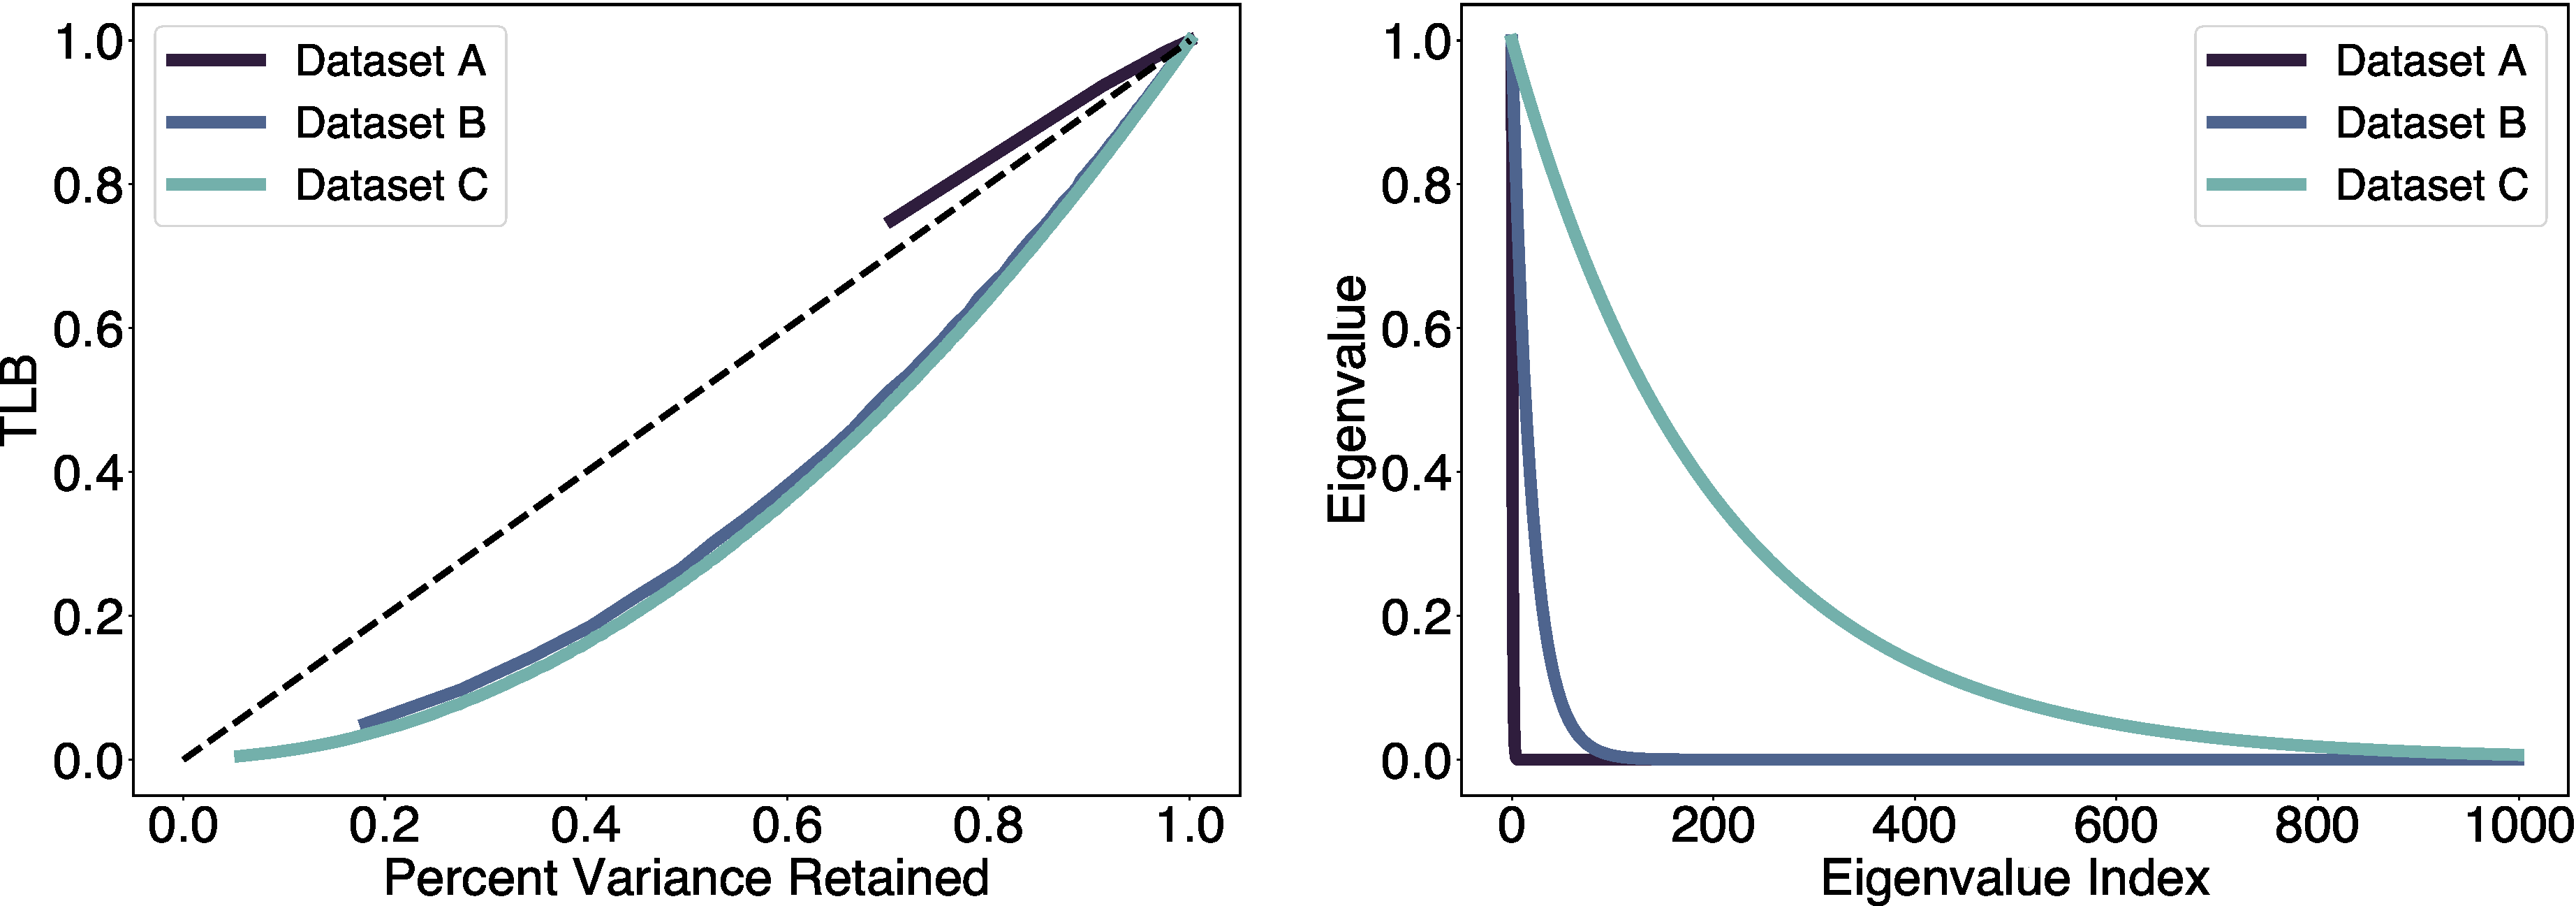
\includegraphics[width= .9\linewidth]{figs/tlb-pca.pdf}

For alternative preservation metrics, we can utilize closed-form confidence intervals~\cite{stats-book,ci1,onlineagg}, or bootstrap-based methods~\cite{bootstrap1,bootstrap2}, which incur higher overhead but can be more generally applied.
\end{comment}

\begin{algorithm}
\begin{algorithmic}[1]
\small
\Statex \textbf{Input:}  
\Statex $X$: sampled data matrix
\Statex $B$: target metric preservation level; default $TLB = 0.98$
\Statex  \hrule 
\Function{compute-transform}{$X, X_i B$}: \label{eq:basis}
	\State \textsc{pca.fit}$(X_i)$
			\Comment{fit PCA on the sample}
	\State Initialize: high $= k_{i-1}$; low $=0$; $k_i= \frac{1}{2}$(low + high); $B_i = 0$
	\While{(low $!=$ high)}
		\State $T_{k_i}, B_i  = \textsc{evaluate-tlb}( X, B, k_i)$
		\If{$B_i \leq B$}  low $= k_i + 1$ 
		\Else  \hspace{0pt} high $= k_i $
		\EndIf
		\State $k_i = \frac{1}{2}$(low + high)
	\EndWhile
	\State $T_{k_i} = $ cached $k_i$-dimensional PCA transform\\
	\Return $T_{k_i}$
\EndFunction
\Statex 
\Function{evaluate-tlb}{$X, B, k$}: \label{eq:eval}
	\State numPairs $= \frac{1}{2}\mvar(\mvar-1)$
	\State $p = 100$
		\Comment{number of pairs to check metric preservation}
	\While{($p < $ numPairs)}
		\State $B_i, B_{lo}, B_{hi} = $ \textsc{tlb}($ X, p, k$)
			 \label{eq:paircheck}
		\If{($B_{lo} > B$ or $B_{hi} < B$)}   \textbf{break}
		\Else \hspace{0pt} pairs $\times$= $ 2$
		\EndIf
	\EndWhile
	\\\Return $B_i$	
\EndFunction
\Statex 
\Function{tlb}{$X, p, k$}: \label{eq:tlbeval}
	\State \textbf{return } mean and 95\%-CI of the $TLB$ after transforming $p$ $d$-dimensional pairs of points from $X$ to dimension $k$. The highest transformation computed thus far is cached to avoid recomputation of the transformation matrix.
\EndFunction

\end{algorithmic}
\caption{Basis Evaluation and Search}
\label{alg:candidate}
\end{algorithm}


\subsection{Progress Estimation}
\label{subsec:pest}
%Given a low dimensional $TLB$-achieving transformation from the evaluation step, DROP must identify the dimensionality $k_i$ and runtime ($r_i$) of the transformation that would be obtained from an additional DROP iteration.
%We refer to this as the $progress estimation$ step.

Recall that the goal of workload-aware DR is to minimize $R + \mathcal{C}_\mvar(k)$ such that $TLB(XT_k) \geq B$, with $R$ denoting total DR (i.e., DROP's) runtime, $T_k$ the $k$-dimensional $TLB$-preserving transformation of data $X$ returned by DROP, and $\mathcal{C}_\mvar(k)$ the workload cost function. 
Therefore, given a $k_i$-dimensional transformation $T_{k_i}$ returned by the evaluation step of DROP's $i^{\text{th}}$ iteration, DROP can compute the value of this objective function by substituting its elapsed runtime for $R$ and $T_{k_i}$ for $T_k$.  
We denote the value of the objective at the end of iteration $i$ as $obj_i$. 

To decide whether to continue iterating to find a lower dimensional transform, we show in  \S\ref{subsec:opt} that DROP must estimate $obj_{i+1}$. To do so, DROP must estimate the runtime required for iteration $i+1$ (which we denote as $r_{i+1}$, where $R=\sum_i r_i$ after $i$ iterations) and the dimensionality of the $TLB$-preserving transformation produced by iteration $i+1$, $k_{i+1}$. 
DROP cannot directly measure $r_{i+1}$ or $k_{i+1}$ without performing iteration $i+1$, thus performs online progress estimation. Specifically, DROP performs online parametric fitting to compute future values based on prior values for $r_{i}$ and $k_i$ (Alg.~\ref{alg:DROP}, l\ref{eq:estimate}). 
By default, given a sample of size $m_i$ in iteration $i$, DROP performs linear extrapolation to estimate $k_{i+1}$ and $r_{i+1}$. The estimate of $r_{i+1}$, for instance, is:

\vspace{-.4cm}
\begin{equation*}
\hat{r}_{i+1} = r_i + \frac{r_i - r_{i-1}}{m_i - m_{i-1}} (m_{i+1} -  m_i).
\end{equation*}

\begin{comment}
\red{
DROP's use of a basic first-order approximation is motivated by the fact that when adding a small number of data samples each iteration, both runtime and resulting lower dimension do not change drastically (i.e., see Fig.~\ref{fig:progressive} after a feasible point is achieved). 
While linear extrapolation acts as a proof-of-concept for progress estimation, the architecture can incorporate more sophisticated functions as needed (\S\ref{sec:relwork}).
}
\end{comment}

\subsection{Cost-Based Optimization}
\label{subsec:opt}

DROP must determine if continued PCA on additional samples will improve overall runtime. 
%We refer to this as the $cost-based optimization$ step. 
Given predictions of the next iteration's runtime ($\hat{r}_{i+1}$) and dimensionality ($\hat{k}_{i+1}$), DROP uses a greedy heuristic to estimate the optimal stopping point.
If the estimated objective value is greater than its current value ($obj_i < \widehat{obj}_{i+1}$), DROP will terminate. 
If DROP's runtime is convex in the number of iterations, we can prove that this condition is the optimal stopping criterion via convexity of composition of convex functions. 
This stopping criterion leads to the following check at each iteration (Alg.\ref{alg:DROP}, l\ref{eq:optimize}): 

\vspace{-.4cm}
\begin{align}
  obj_i &< \widehat{obj}_{i+1} \nonumber \\
  \mathcal{C}_\mvar(k_i) + \sum_{j=0}^i r_j &< \mathcal{C}_\mvar(\hat{k}_{i+1}) + \sum_{j=0}^{i} r_j + \hat{r}_{i+1} \nonumber \\
  % \mathcal{C}_\mvar(k_i)  &< \mathcal{C}_\mvar(\hat{k}_{i+1}) + \hat{r}_{i+1}  \nonumber \\
  \mathcal{C}_\mvar(k_i) - \mathcal{C}_\mvar(\hat{k}_{i+1}) &< \hat{r}_{i+1}  \label{eq:check}
\end{align}

DROP terminates when the projected time of the next iteration exceeds the estimated downstream runtime benefit. 
%Absent $\mathcal{C}_d$, we default to execution until convergence (i.e, $k$ plateaus), and show the cost of doing so in \S\ref{sec:experiments}.


\begin{comment}
\red{In the general case as the rate of decrease in dimension ($k_i$) is data dependent, thus convexity is not guaranteed. 
Should $k_i$ plateau before continued decrease, DROP will terminate prematurely. 
This occurs during DROP's first iterations if sufficient data to meet the $TLB$ threshold at a dimension lower than $\dvar$ has not been sampled (SmallKitchenAppliances in Fig.~\ref{fig:progressive}).
Thus, optimization is only enabled once a feasible point is attained, as we prioritize accuracy over runtime (i.e., $0.3$ for SmallKitchenAppliances).
We show the implications of this decision in DROP in \S\ref{subsec:arch}.%, and in the streaming setting in the extended manuscript.
}
\end{comment}

\subsection{Choice of PCA Subroutine}
\label{subsec:pcaroutine}

The most straightforward means of implementing PCA via SVD in DROP is computationally inefficient compared to DR alternatives (\S\ref{sec:background}).  
DROP computes PCA via a randomized SVD algorithm from~\cite{tropp} (SVD-Halko).
Alternative efficient methods for PCA exist (i.e., PPCA, which we also provide), but we found that SVD-Halko is asymptotically of the same running time as techniques used in practice, is straightforward to implement, is $2.5-28\times$ faster than our baseline implementations of SVD-based PCA, PPCA, and Oja's method, and does not require hyperparameter tuning for batch size, learning rate, or convergence criteria.  
%While SVD-Halko is not as efficient as other techniques with respect to communication complexity as in~\cite{ppca-sigmod}, or convergence rate as in~\cite{re-new}, these techniques can be easily substituted for SVD-Halko in DROP's architecture.
%%%%We demonstrate this by implementing multiple alternatives in \S\ref{subsec:pcaexp}.
%%%%\red{Further, we also demonstrate that this implementation is competitive with the widely used SciPy Python library~\cite{scipy}}.

\begin{comment}
\begin{algorithm}[t]
\begin{algorithmic}
\State \textbf{Input:}  \\
$H$: concatenation of previous transformation matrices \\
$T$: new sample's transformation \\
 points to sample per iteration; default 5\% \\
 
\\ \hrule

\Function{distill}{$H, T$}:
	\State $H \gets [H | T]$
		\Comment{Horizontal concatenation to update history}
	\State $U, \Sigma, V^\intercal \gets \textsc{SVD}(H)$ 
				\Comment{$U$ is a basis for the range of $T$}
	\State $T \gets U[:,\textsc{num-columns(T)}]$
	\\\Return{$T$}
\EndFunction
\end{algorithmic}
\caption{Work Reuse}
\label{alg:reuse}
\end{algorithm} 
\end{comment}

\subsection{Work Reuse}
\label{subsec:reuse}

A natural question arises due to DROP's iterative architecture: can we combine information across each sample's transformations without computing PCA over the union of the data samples? 
Stochastic PCA methods enable work reuse across samples as they iteratively refine a single transformation matrix, but other methods do not.
%We propose an algorithm that allows reuse of previous work when utilizing arbitrary PCA routines with DROP.
DROP uses two insights to enable work reuse over any PCA routine.

First, given PCA transformation matrices $T_1$ and $T_2$, their horizontal concatenation $H = [T_1 | T_2]$ is a transformation into the union of their range spaces.
Second, principal components returned from running PCA on repeated data samples generally concentrate to the true top principal components for datasets with rapid spectrum drop off.
Work reuse thus proceeds as follows:
DROP maintains a transformation history consisting of the horizontal concatenation of all transformations to this point, computes the SVD of this matrix, and returns the first $k$ columns as the transformation matrix. 

Although this requires an SVD computation, computational overhead is dependent on the size of the history matrix, not the dataset size.
This size is proportional to the original dimensionality $\dvar$ and size of lower dimensional transformations, which are in turn proportional to the data's intrinsic dimensionality and the $TLB$ constraint.
As preserving \emph{all history} can be expensive in practice, 
DROP periodically shrinks the history matrix using DR via PCA. 
We validate the benefit of using work reuse---up to \red{15\%} on real-world data---in \S\ref{sec:experiments}.

